\chapter{Prototypische Implementierung}
\label{chap:impl}
Dieses Kapitel widmet sich der prototypischen Implementierung der im vorigen Kapitel vorgestellten Konzeption der Publish/Subscribe-Komponente von \ac{m2etis}. Bevor der Aufbau dieser Komponente beschrieben wird, wird die gewählte Entwicklungsumgebung (Programmiersprache und gewähltes \ac{p2p}-Netzwerk) beschrieben. Der Zugriff auf das Publish/Subscribe-System zeigt die einfache Schnittstelle aus Benutzersicht. Die vom Optimierungsschritt zu erstellenden beziehungsweise zu verändernden Dateien werden im darauffolgenden Kapitel beschrieben. Details aus der Implementierung schließen dieses Kapitel ab.

\section{Wahl der Entwicklungsumgebung}
Als Programmiersprache wird C++ gewählt, da diese Sprache die gesamte Bandbreite der Softwareentwicklung anbietet und sowohl den Zugriff auf die Hardware des Computers als auch die Entwicklung von großen Systemen begünstigt. C++ legt auch einen Schwerpunkt auf die Sprachmittel zur Entwicklung von Bibliotheken und favorisiert dadurch verallgemeinerte Mechanismen gegenüber in die Sprache integrierten Einzellösungen für typische Problemstellungen. Eine der Stärken von C++ -- als Multiparadigmensprache -- ist dabei die Kombination von effizienter, maschinennaher Programmierung mit mächtigen Sprachmitteln zur Anwendungsentwicklung. Dabei kommt in dieser Arbeit vor allem die \acf{tmp} zum Zuge: Eine Technik, die eine nahezu kompromisslose Verbindung von Effizienz und Abstraktion erlaubt. Ansätze dieser Technik sind in \Fref[plain]{chap:impl_tmp} im Anhang dieser Arbeit beschrieben.

Mit der Festlegung auf C++ muss auch die Implementierung des p2p-Netzwerkes durch C++ ansprechbar sein. Das bedeutet, das Netzwerk muss als C- oder C++-Bibliothek vorliegen. Chimera \cite{Allen2006Chimera} ist der Nachfolger von Tapestry und wird auf der Homepage\footnote{siehe \url{http://current.cs.ucsb.edu/projects/chimera/index.html} (26.\,11.\,2010)} folgendermaßen beschrieben: 
\selectlanguage{english}
\begin{quote}
Chimera is a light-weight C implementation of a \enquote{next-generation} structured overlay that provides similar functionality as prefix-routing protocols Tapestry and Pastry.  Chimera gains simplicity and robustness from its use of Pastry's leafsets, and efficient routing from Tapestry's locality algorithms.  In addition to these properties, Chimera also provides efficient detection of node and network failures, and reroutes messages around them to maintain connectivity and throughput.  
\end{quote}
\selectlanguage{ngerman} 

Pastry\footnote{\url{http://www.freepastry.org} (26.\,11.\,2010)} und Tapestry sind als Java-Bibliotheken verfügbar und die Entwicklung von Tapestry wurde mit Version 2.01 eingestellt. Chimeras frei verfügbarer Code (veröffentlicht unter GPL) und die Kompabilität mit der generischen KBR-API sprechen weiterhin für Chimera. Bei gravierenden Problemen kann es somit durch ein anderes Netzwerk ausgetauscht werden, ohne dass diese Änderung großen Einfluss auf die restlichen Komponenten von \ac{m2etis} hat. 


\section{Aufbau der Publish/Subscribe-Komponente}

Das UML-Klassendiagramms in \Fref[plain]{fig:uml} spiegelt den groben Aufbau der Komponenten wieder und zeigt die Verbindung der wichtigsten Klassen. Auf die Darstellung von Hilfskonstrukten wird der Übersichtlichkeit halber verzichtet. Als erster Schritt wird die Anbindung an das \ac{p2p}-Netzwerk beschrieben. Danach wird -- ausgehend von der Applikation -- die Implementierung des Publish/Subscribe-Systems erläutert. Angewandte Techniken wie \ac{tmp} oder \emph{policy based}-Design werden im Anhang dieser Arbeit beschrieben. Sie werden benötigt um den zusätzlichen Verwaltungsaufwand zur Laufzeit durch geschickte Anwendung des zur Übersetzungszeit vorhandenen Wissens zu minimieren. Das nutzbare Wissen umfasst beispielsweise die Typen der Events oder die zur Optimierung ausgewählten Strategien und deren Besonderheiten.

\texttt{P2PInterface} ist eine abstrakte Basisklasse und repräsentiert die in \Fref[plain]{chap:grundlagen:api} beschriebene \ac{kbr}-API. Aktuell wird diese durch die Klasse \texttt{ChimeraWrapper} implementiert, welche über die Klasse \texttt{ChimeraWrapperImpl} Zugriff auf das Netzwerk Chimera bietet. Hier wurde das \enquote{PIMPL}-Pattern angewandt, mit dem die eigentliche Implementierung versteckt werden kann \cite{Alexandrescu2001Modern}. Damit werden die Implementierungsdetails, wie interne Datentypen oder Methoden, vor dem Nutzer versteckt und müssen demnach nicht im zu inkludierenden Header angegeben werden. Diese können nun nach Belieben geändert werden, ohne dass der Nutzer neukompilieren muss, da sich die Schnittstelle nicht verändert. Als Nebeneffekt sinkt die Übersetzungzeit, da insgesamt weniger Header inkludiert und geparst werden müssen.

Zur Vereinfachung werden sämtliche Identifikationsdaten, zum Beispiel die Adresse eines Knotens, des Netzwerkes als \texttt{std::string} repräsentiert. Dies entbindet den Entwickler der Implementierung weiterer Wrapperklassen von komplexen Hilfskonstrukten. Eventuell muss daher in der Implementierungsklasse (in unserem Fall \texttt{ChimeraWrapperImpl} eine zusätzliche Indirektion eingeführt werden. Zur eigentlichen Nachrichtenübertragung wird der Datentyp \texttt{std::vector$<$char$>$}, die objektorientierte Version eines \texttt{char*}, bereitgestellt. Neben der einfacheren Zugriffsweise bietet dies zusätzlichen Schutz beispielsweise gegen einen Pufferüberlauf.\\
Weitere Netzwerke können auf einfache Art und Weise durch entsprechende Wrapperklassen eingebunden werden.

\begin{figure}[htbp]
\centering
\resizebox{\textwidth}{!}{%
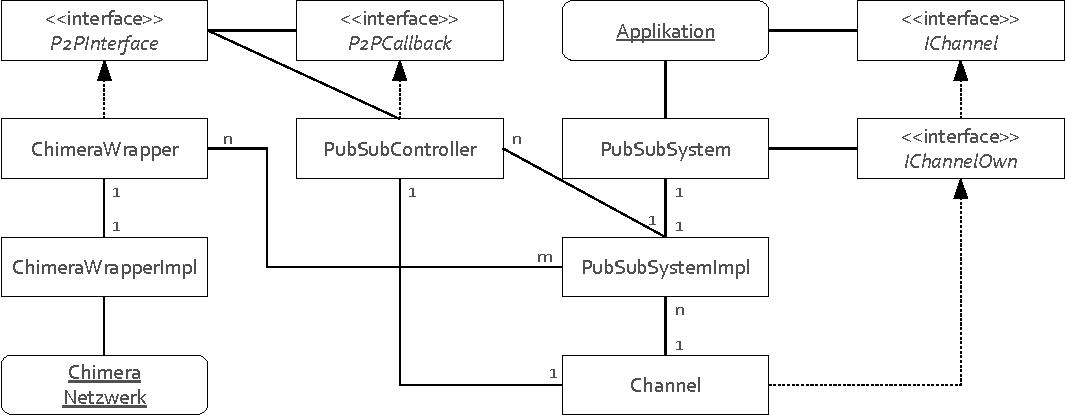
\includegraphics{grafics/uml.pdf}}
\caption{Vereinfachtes Klassendiagramm des Frameworks}
\label{fig:uml}
\end{figure}

Die \texttt{Applikation} greift auf das Publish/Subscribe-System über den Singleton \texttt{PubSub\-Sytem} zu. Beiden ist der optimierte \texttt{Channel} nur über die abstrakten Basisklassen \texttt{IChannel} beziehungsweise \texttt{IChannelOwn} zugänglich. Diese sind in \Fref[plain]{lst:interface_channel} dargestellt und bieten lediglich die drei üblichen Methoden\footnote{\texttt{subscribe}, \texttt{unsubscribe} und \texttt{publish}} für Publish/Subscribe-Systeme an. Sie verdecken dadurch die Komplexität der Klasse \texttt{Channel} vor dem Benutzer. Bei der Anmeldung an einem Kanal muss ein Funktionspointer vom Typ \texttt{app\_deliver\_func} übergeben werden. Diesem übergibt das Publish/Subscribe-System eine empfangene Nachricht und liefert damit die Events an die Applikation aus. Der Anmeldung kann ebenfalls ein Prädikat zur Filterung übergeben werden, falls die gewählten Strategien dies unterstützen. \texttt{Channel} selbst ist eine mit policy-based Design erstellte Templateklasse\footnote{siehe \Fref{chap:impl_tmp} im Anhang zur Erklärung} und bekommt die verschiedenen Strategien -- in \Fref{fig:uml} ebenfalls nicht dargestellt -- als Policies übergeben. \ac{tmp} ermöglicht zudem, jede \texttt{Channel}-Instanz auf die gewählten Policies abzustimmen. Weiterhin wird für jeden \texttt{Channel} ein optimierter Header erzeugt, dessen Größe an Nutzlast für Verwaltungsdaten von den gewählten Policies abhängig ist. Durch diese Maßnahmen wird der Overhead zur Laufzeit stark reduziert. 

\lstinputlisting[caption={Schnittstellen für die Klasse \texttt{Channel}}, label=lst:interface_channel, float=!t]{listings/interface_channel.h}

Die Klasse \texttt{PubSubController} implementiert das Interface \texttt{P2PCallback} und kann sich somit für die Callbacks des Netzwerkes registrieren. Der PubSubController ist die Schnittstelle des Publish/Subscribe-Systems mit dem \ac{p2p}-Netzwerk und bietet die benötigte Funktionalität für die Klasse Channel. Zudem werden die ankommenden Nachrichten in deliver über eine Queue und einen Dispatch-Thread an die einzelnen Kanäle verteilt. 

\texttt{PubSubSystemImpl} ist eine der generierten Klassen (siehe nächstes Kapitel) und kennt die verschiedenen Netzwerkwrapper (in \Fref{fig:uml} ist dies \texttt{ChimeraWrapper}). Aktuell besitzt sie für jeden optimierten \texttt{Channel} einen Pointer auf \texttt{IChannelOwn} als Klassenvariable. Auf diese hat die Klasse \texttt{PubSubSystem} als \texttt{friend class}\footnote{\enquote{friend} ist eine besondere Beziehung zwischen zwei Klassen} freien Zugriff und kann die Methodenaufrufe an der Publish/Subscribe-API an die einzelnen Instanzen. Für jedes genutzte Netzwerk instantiiert \texttt{PubSubSystemImpl} einen eigenen \texttt{PubSubController} und übergibt diesen an die entsprechenden Kanäle. Mit verschiedenen Instanzen der Klasse \texttt{PubSubController} können somit auch verschiedene Netzwerke angesprochen und entsprechend der Optimierungsmetriken für verschiedene Kanäle genutzt werden.

Die UML-Beschreibung der als \emph{Singleton} implementierten Klasse \texttt{PubSubSystem} -- die zur Interaktion mit \ac{m2etis} dem Nutzer zur Verfügung steht -- ist in \Fref{fig:uml_pubsubsystem} dargestellt. Zur Vereinfachung sind lediglich die \texttt{public} verfügbaren Methoden angegeben. Die Schnittstelle der Klasse erlaubt \emph{method chaining}, den einfachen Aufruf mehrerer Methoden hintereinander und erfordert meist die Angabe des Kanals -- kodiert in ein \texttt{enum} des Typs \texttt{ChannelList}, welches im nächsten Abschnitt genauer beschrieben wird.  Durch die überladene Methode \texttt{init}, wird der Eintritt des Knotens in das \ac{p2p}-Netzwerk angestoßen. Der erste Knoten baut das Netzwerk auf, während die restlichen Knoten nur über bekannte Knoten in das Netzwerk eintreten können. Nur durch Methoden der Klasse \texttt{PubSubSystem} kann sich ein Knoten für einen Kanal an- beziehungsweise abmelden. Über ein \emph{Handle} auf einen Kanal lässst sich jedoch nur publizieren. Das Beispiel in \Fref[plain]{lst:pubsub_usage} zeigt, wie einfach diese Schnittstelle benutzt werden kann.

\begin{figure}[htbp]
\centering
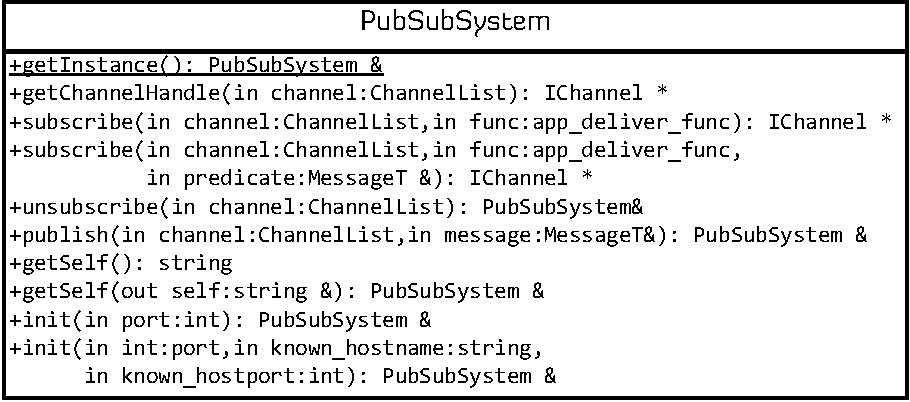
\includegraphics{grafics/uml_pubsubsystem.pdf}
\caption{UML-Beschreibung der Klasse \texttt{PubSubSystem}}
\label{fig:uml_pubsubsystem}
\end{figure}

Dank der strikten Aufteilung der Klassen beim Netzwerk und dem Publish/Subscribe-System wird die Nutzerfreundlichkeit des Frameworks aus Entwicklersicht ermöglicht, wie es das Codebeispiel im nächsten Abschnitt darlegt. Hier ist deutlich zu sehen, dass der Nutzer keinerlei Wissen über das genutzte Netzwerk noch über die zur Optimierung herangezogenen Strategien haben muss, um das System benutzen zu können.

\section{Zugriff auf M$^2$etis aus Benutzersicht}
Das \Fref[plain]{lst:pubsub_usage} zeigt den Zugriff der Applikation auf das Publish/Subscribe-System. Der Code erzeugt drei Knoten, die mit dem System arbeiten. Der erste Knoten sendet Nachrichten auf dem Kanal \texttt{ANY\_ALL}\footnote{Der Name \enquote{ANY\_ALL} suggeriert, dass hier jegliche Art von Nachrichten an alle Knoten verteilt werden.}, für den sich die beiden anderen Knoten anmelden. In den Zeilen 10 bis 12 ist die Empfangsfunktion definiert, welche dem System bei Anmeldungen übergeben werden muss. Diese Funktion wird in den Zeilen 18 und 21 mittels \texttt{boost::bind} an die benötigte Signatur angepasst und mit Metadaten (hier der Knotenname) angereichert. Das System wird in den Zeilen 15 und 16 initialisiert und ein Handle auf den Kanal \texttt{ANY\_ALL} erlangt. Die Anmeldung der Knoten erfolgt in den Zeilen 19 und 22, mit Angabe eines im Netzwerk bekannten Knoten zum Einstieg in das Netzwerk und der Empfangsfunktion. In den Zeilen 24\,-\,27 wird in einer Endlosschleife eine Nachricht über das Handle in das System gebracht und fünf Sekunden geschlafen.


\lstinputlisting[caption={Zugriff auf M$^2$etis aus Benutzersicht}, label=lst:pubsub_usage, float=!t]{listings/pubsub_usage.cpp}

Dieses Codebeispiel zeigt deutlich die Kapselung des komplexen optimierten Publish/\-Subscribe-Systems und dessen einfache und unkomplizierte Handhabbarkeit. Über \texttt{boost::bind} können beliebige Methoden an die Signatur der Empfangsfunktion angepasst werden. Daher muss die Applikation einerseits nicht von einer abstrakten Basisklasse abgeleitet sein und andererseits bleibt die eigentliche Empfangsfunktion anpassbar, wie es im Codebeispiel dargestellt ist.

Nach diesem Beispiel zur einfacher Schnittstellennutzung, wird im folgenden auf die im Optimierungsschritt\footnote{Schritt 2 in \Fref{fig:metis_aufbau}} zu erstellenden Klassen eingegangen.

\section{Anforderungen an den Optimierungsschritt}
Die Dateien und Klassen müssen in der richtigen Reihenfolge generiert und angepasst werden um die verschiedenen Kanäle zu erzeugen und mit dem Netzwerk zu verbinden. \Fref{fig:reihenfolge} zeigt diese Reihenfolge der nun vorgestellten Dateien.

\begin{figure}[!h]
\centering
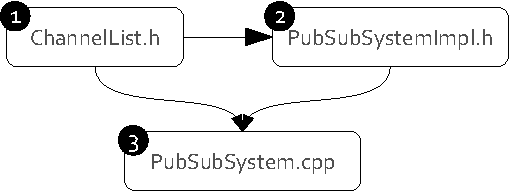
\includegraphics{grafics/reihenfolge.pdf}
\caption{Erstellungsreihenfolge der Dateien im Optimierungsschritt}
\label{fig:reihenfolge}
\end{figure}


\subsubsection*{\texttt{ChannelList.h}}
Der \ac{m2etis}-Optimierer muss die Datei \texttt{ChannelList.h} komplett generieren und alle vorhandenen Kanäle -- die je einem Eventtyp entsprechen -- benennen und im \texttt{enum} eintragen, wie es \Fref{lst:channellist} darstellt. Die Einträge dienen der Auswahl des Kanals bei der Kommunikation mit dem \texttt{PubSubSytem}. Durch das \texttt{enum} wird ein zur Laufzeit einfach zu überprüfendes Mapping auf die eigentliche Implementierung des Kanal ermöglicht und es ist nicht möglich einen, dem System unbekannten, Kanal anzufordern.

\lstinputlisting[caption={Beispiel für die generierte Datei \texttt{ChannelList.h}}, label=lst:channellist, float=!t]{listings/channellist.h}


\subsubsection*{\texttt{PubSubSystemImpl.h}}
\texttt{PubSubSystemImpl} ist -- wie schon beschrieben -- die Implementierung der offentlichen Schnittstelle für Nutzer von \ac{m2etis}. Sie muss komplett generiert werden, da sie Zugriff auf alle zur Optimierung genutzten Strategien hat und damit die daraus erzeugten optimierten Instanzen der Templateklasse \texttt{Channel} als Klassenvariablen besitzt.

\Fref[plain]{lst:pubsubsystemimpl} zeigt einen Ausschnitt dieser generierten Datei. In den Zeilen 3 und 4 wurden vom Optimizer zwei optimierte Kanaltypen erstellt. Die Liste der Policys wurde aus Gründen der Übersichtlichekeit ausgelassen. In der aktuellen Version sind die optimierten Kanäle Klassenvariablen, wie in den Zeilen 18 bis 20 sichtbar ist.  Diese Variablen werden in der Initialisierungsliste der Konstruktors (Zeile 9) erstellt und erhalten über den \texttt{PubSubController} Zugriff auf das Netzwerk. Es ist offensichtlich, dass der Optimierer verschiedene Netzwerke mit den einzelnen Instanzen der Klasse \texttt{Channel} verbinden kann.

\lstinputlisting[caption={Ausschnitt der Klasse \texttt{PubSubSystemImpl}}, label=lst:pubsubsystemimpl, float=h!t]{listings/pubsubsystemimpl.h}


\subsubsection*{\texttt{PubSubSystem.cpp}}
Die Klasse \texttt{PubSubSystemImpl} und damit auch die optimierten Kanäle werden erst im Optimierungsschritt erzeugt. Die Klasse \texttt{PubSubSystem} hat jedoch direkten Zugriff auf in \texttt{PubSubSystemImpl} enthaltenen Kanäle und muss daher ebenfalls im Optimerungsschritt generiert werden. \Fref[plain]{lst:pubsubsystem} zeigt mit der Methode \texttt{getChannelHandle} einen Ausschnitt des generierten Codes. \texttt{impl\_} ist eine Klassenvariabele auf eine Instanz von \texttt{PubSubSystemImpl}. Das Codebeispiel zeigt, das \texttt{PubSubSystem} als Dispatcher arbeitet und die entsprechenden Kanäle anhand der \texttt{ChannelList} auswählt. Dieser Zugriff ist nur möglich, das \texttt{PubSubSystem} als \texttt{friend} der Klasse \texttt{PubSubSystemImpl} (\Fref[plain]{lst:pubsubsystemimpl} Zeile 7) definiert ist.

\lstinputlisting[caption={Ausschnitt des zu generierenden Abschnittes von \texttt{PubSubSystem.cpp}}, label=lst:pubsubsystem, float=!t]{listings/pubsubsystem.cpp}

\section{Implementierungsdetails der Klasse \texttt{Channel}}
In diesem Abschnitt werden Ausschnitte der Klasse \texttt{Channel} gezeigt um damit verschiedene Implementierungsdetails aufzuzeigen. Als erstes wird die Umsetzung eines Teils des Verarbeitungsmodells beim Empfang einer \emph{Pubslish}-Nachricht in \texttt{deliver} gezeigt. \Fref[plain]{fig:processing_deliver_ovpd} zeigt diesen Teil des Verarbeitungsmodells als Ausschnitt und in \Fref{lst:ovpd} ist der zugehörige Codeausschnitt der Klasse \texttt{Channel} dargestellt. In der Zeile 2 werden die Verwaltungsinformationen der Nachricht ausgelesen und in einem \texttt{Header} gespeichert.  Die Schleife -- beginnend in Zeile 6 -- zeigt die weitere Verarbeitung der \emph{freigegebenen} Nachrichten bishin zur Übergabe an die Applikation (Zeile 16). Die gewählte Strategie der Policy \emph{Reihenfolge} -- hier über \texttt{Order} ansprechbar -- bekommt die zu bearbeitende Nachricht mitsamt einiger Verwaltungsinformationen übergeben. Der Rückgabewert dieser Methode ist eine Liste von \emph{freigegebenen} Nachrichten zusammen mit den weiter benötigten Verwaltunsginformationen. Anhand diesen, kann die Strategie zur \emph{Validierung} -- über \texttt{Validity} ansprechbar -- in Zeile 13 prüfen ob die Nachricht gültig ist oder verworfen werden muss (Zeile 14). Als letzter Schritt vor der Übergabe der Nachricht an die Applikation, kann in Zeile 15, der Event oder dessen Auswirkung auf die virtuelle Welt abgespeichert werden.

\lstinputlisting[caption={Verarbeitung einer \emph{Publish}-Nachricht in \texttt{deliver}}, label=lst:ovpd, float=t]{listings/ovpd.cpp}

\begin{figure}[htbp]
\centering
\resizebox{\textwidth}{!}{%
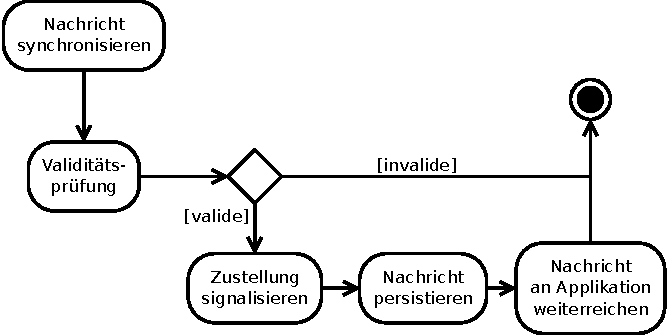
\includegraphics{grafics/processing_deliver_ovpd.pdf}}
\caption{Ausschnitt der Nachrichtenverarbeitung in \texttt{deliver}}
\label{fig:processing_deliver_ovpd}
\end{figure}

Das nächste Beispiel zeigt in \Fref{lst:publish} die Erstellung einer \emph{Publish}-Nachricht und allgemein den Versand einer Nachricht. In der Methode \texttt{publish} werden die Verwaltungsinformationen aller Strategien abgefragt. Der \emph{Filterung} wird zusätzlich die Nachricht übergeben, anhand der die gewählte Strategie Metadaten zu Filterung erzeugen kann. In Zeile 10 wird der ersteller \texttt{Header} und die Nachricht an \texttt{sendMessages} unter Angabe des Types (\texttt{publish\_}) übergeben.\\
Im ersten Abschnitt dieser Methode (Zeilen 14 bis 18) wird der übergebene Nachrichtentyp in einen generischen Typ umgewandelt. Der Nachrichtnentyp entspricht der Nachrichtennummer im Netzwerk und muss daher für die Verteilungspolicy umgewandelt werden. Im zweiten Abschnitt (Zeilen 20 bis 25) wird die eigentliche Nachricht erstellt und verschlüsselt.\\
Für den Fall einer \emph{Publish}-Nachricht wird im dritten Abschnitt (Zeilen 27 bis 34) wird ermittelt ob die Verteilungsstrategie eine Filterung der Empfängerliste wünscht.\\
Im letzten Abschnitt dieser Methode (Zeilen 36 bis 40), wird die Liste der Empfänger von der Verteilungsstrategie errechnet und in Zeile 39 -- nach erfolgter Prüfung -- über das Netzwerk versandt.

\lstinputlisting[caption={Versenden einer \emph{Publish}-Nachricht}, label=lst:publish, float=t]{listings/publish.cpp}

Das nächste \Fref{lst:header} zeigt Auszüge der, an die gewählten Strategien angepasste, Klasse \texttt{Header}, die als Klasse innerhalb der Klasse \texttt{Channel} implementiert ist und damit Zugriff auf die, der Klasse \texttt{Channel} übergebenen, Policys hat. Die Größe des Feldes für Verwaltungsinformationen wird anhand der Werte der einzelnen Strategien berechnet. \texttt{KeySize} ist die Länge der Stringrepräsentation eines Schlüssels im Netzwerk und wird der Klasse \texttt{Channel} als Policy übergeben. Jede Strategie \emph{muss} über das Feld \texttt{size} zur Übersetzungszeit angeben, wie viele \texttt{chars} sie zur Speicherung ihrer Metadaten pro Nachricht benötigt. Damit kann die benötigte Größe in Zeile 11 berechnet werden und ein entsprechendes \texttt{char[]} in Zeile 13 erstellt werden. Das restliche Codebespiel zeigt einige der Zugriffsmethoden auf die einzelnen Metadaten. Auch hier ist ersichtlich, dass diese bereits zur Übersetzungszeit mit exakten Werten erstellt werden und somit effektiv gegen Pufferüberlauf schützen. 

\lstinputlisting[caption={An die gewählten Strategien angepasste Klasse \texttt{Header}}, label=lst:header, float=t]{listings/header.h}

